% !TEX root = ../my-thesis.tex
%
\chapter{Introduction}
\label{sec:intro}

\cleanchapterquote{TODO}{TODO}{(TODO)}

% ---------------------------------------
\section{From seven sisters to a powerhouse of astronomy}
\label{sec:intro:intro}

\begin{figure}[tb]
	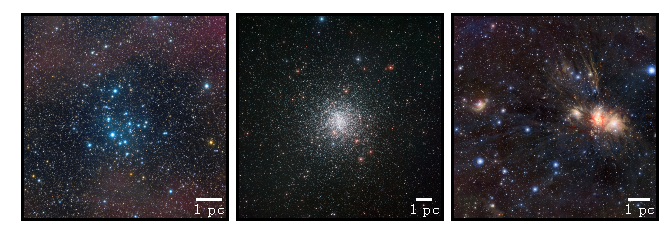
\includegraphics[width=\textwidth]{fig/c1/oc_gc_mg_comparison.pdf}
	\caption{TODO}
	\label{fig:intro:intro:comparison}
\end{figure}


% ---------------------------------------
\section{The history and techniques of open cluster observations}
\label{sec:intro:history}

\blindtext

% Plot of the pleiades
\begin{figure}[tb]
	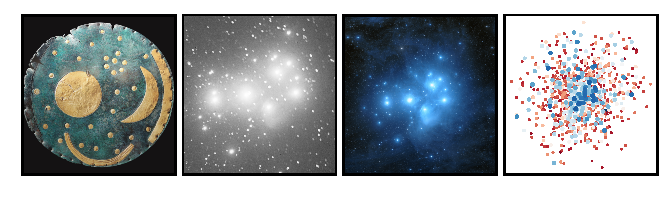
\includegraphics[width=\textwidth]{fig/c1/pleiades.pdf}
	\caption{TODO}
	\label{fig:intro:history:pleiades}
\end{figure}

% Plot of catalogues of OCs
\begin{figure}[htb]
	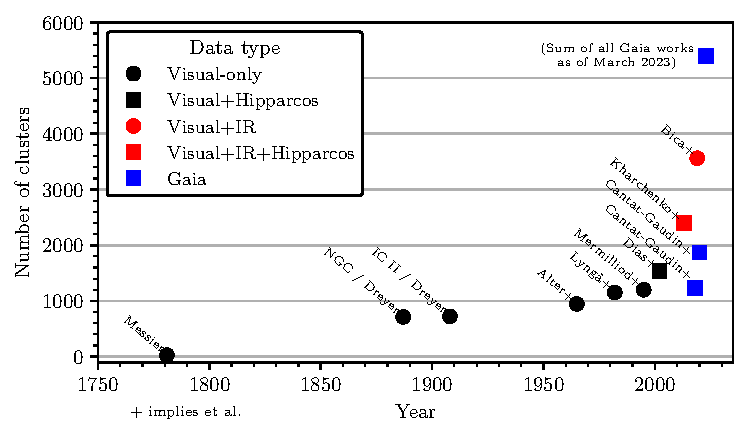
\includegraphics[width=\textwidth]{fig/c1/catalogues.pdf}
	\caption{TODO}
	\label{fig:intro::history:catalogues}
\end{figure}


% Plot of reported OCs
\begin{figure}[htb]
	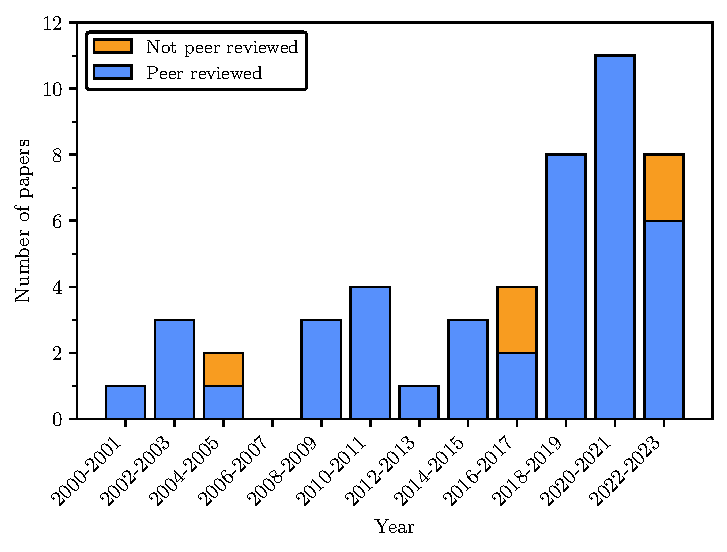
\includegraphics[width=\textwidth]{fig/c1/papers.pdf}
	\caption{TODO}
	\label{fig:intro:history:papers}
\end{figure}


% ---------------------------------------
\section{The \gaia\ revolution in open cluster science}


% ---------------------------------------
\section{Some theoretical background into star clusters}


% ---------------------------------------
\section{Thesis structure}
\label{sec:intro:structure}

\textbf{Chapter \ref{sec:intro}} \\[0.2em]
\blindtext

\textbf{Chapter \ref{sec:intro}} \\[0.2em]
\blindtext

\textbf{Chapter \ref{sec:intro}} \\[0.2em]
\blindtext

\textbf{Chapter \ref{sec:intro}} \\[0.2em]
\blindtext

\textbf{Chapter \ref{sec:intro}} \\[0.2em]
\blindtext
